\chapter{Introduction}
\fxnote{Maybe better chapter/subchapter titles}
In 2019 the population in the world reached 7.7 billion people, which is an increase of one billion over the past twelve years. According to The United Nations Department of Economic and Social Affairs’ (UN DESA) median scenario the growth is expected to continue reaching 9.7 billon in 2050. \citep{UNDEASHightlights} 

To be able to adapt infrastructures to this population growth it is necessary to predict where these people will settle. While UN DESA provides this information on a national level \citep{NationalPop}, it is more ideal with a more nuanced picture, since most planning is based on local or regional scale spatial projections. \citep{WhyDetailedPop}

Other researchers (SEDAC, CISC) have used simulations to distribute the population within each country as raster layers. However due to the high resolution and/or small scales, visually comparing these raster datasets is a time-consuming task. The purpose of this project is to create a tool allowing fast and easy comparison of such raster datasets, focusing on the use case of population projections.

%Evt noget om at det vil være ekstra interessant at have områderne med stor vækst som case - tilføj her, hvis der skal argumenteres for en case senere

\section{Problem statement}

To explore the possibilities for creating such a comparison tool the following research question have been defined:

\textbf{How can population rasters be visualized and compared efficiently and effectively?}

This broad main question will be answered by answering the following three subquestions:

\textit{Which conventions exist for visualization of population projections?}

\textit{Which functionalities are relevant for comparing different rasters?}

\textit{How can a responsive user experience be ensured, when loading and visualizing large raster dataset?}


\section{Limitations}\label{Lim}

Determining relevant functionalities and the responsiveness would ideally have been done with user testing.  However it was determined that both the creation of the tool and a scientific approach to user testing would require too much time.
Therefore the tool creation got prioritised and other evaluation methods not involving users were chosen. This is expanded upon in section \ref{Eval}

\section{Target audience}\label{TA}

The target audience for this project is academic researchers. It is meant as a tool for these researchers to be able to quickly compare different population projections. 

This prototype of the tool has only been created for internal use by single individuals. It will therefore not be created with multiple users in mind and there will be no considerations for security.


The tool is also created with only computers in mind, so it will not be optimized for smartphone users. 

Alternative target audiences are discussed in section x.

\section{Report structure}

\fxnote{ADD: quick overview of what the solution is going to be, what is population projections, SSP}

%The report have been divided into three parts. The first part is the literature review, which will address the first two subquestions and also present the two projections visualised in this project. Chapter x explores which conventions there exist for population projections, while the relevant functionalities for raster comparison are detailed in chapter x. Lastly chapter x will give an overview of the population projection SEDAC and CICS, which will be used as case for comparison.
%
%The second part is addressing the last subquestion. First there is a definition of how a "responsive user experience" has been defined. Then different methods of visualising raster datasets are being tested in chapter x. Based on these initial tests a method will chosen, which will be evaluated in the next section.
%
%The last part starts with a discussion in chapter x of the results of the previous part. This is then followed by the last two chapters x and x, which are the conclusion and future work.  

%Part I: Litterature review
%- Conventions, what are relevant functionalities, Explaining the two case projections
%
%Part II: Choice of method
%- Test of different methods 
%
%Part III: Discussion 

The report has been divided into three parts; design, development and evaluation.




In the design part the thought process behind the design of the solution is explained.
It starts with some background information about the case data in chapter x, raster formatting in chapter x and chapter x about how the raster data currently is being compared. 
\fxerror{Add these three to figure -case,raster,current}
\begin{figure} [H]
	\centering
	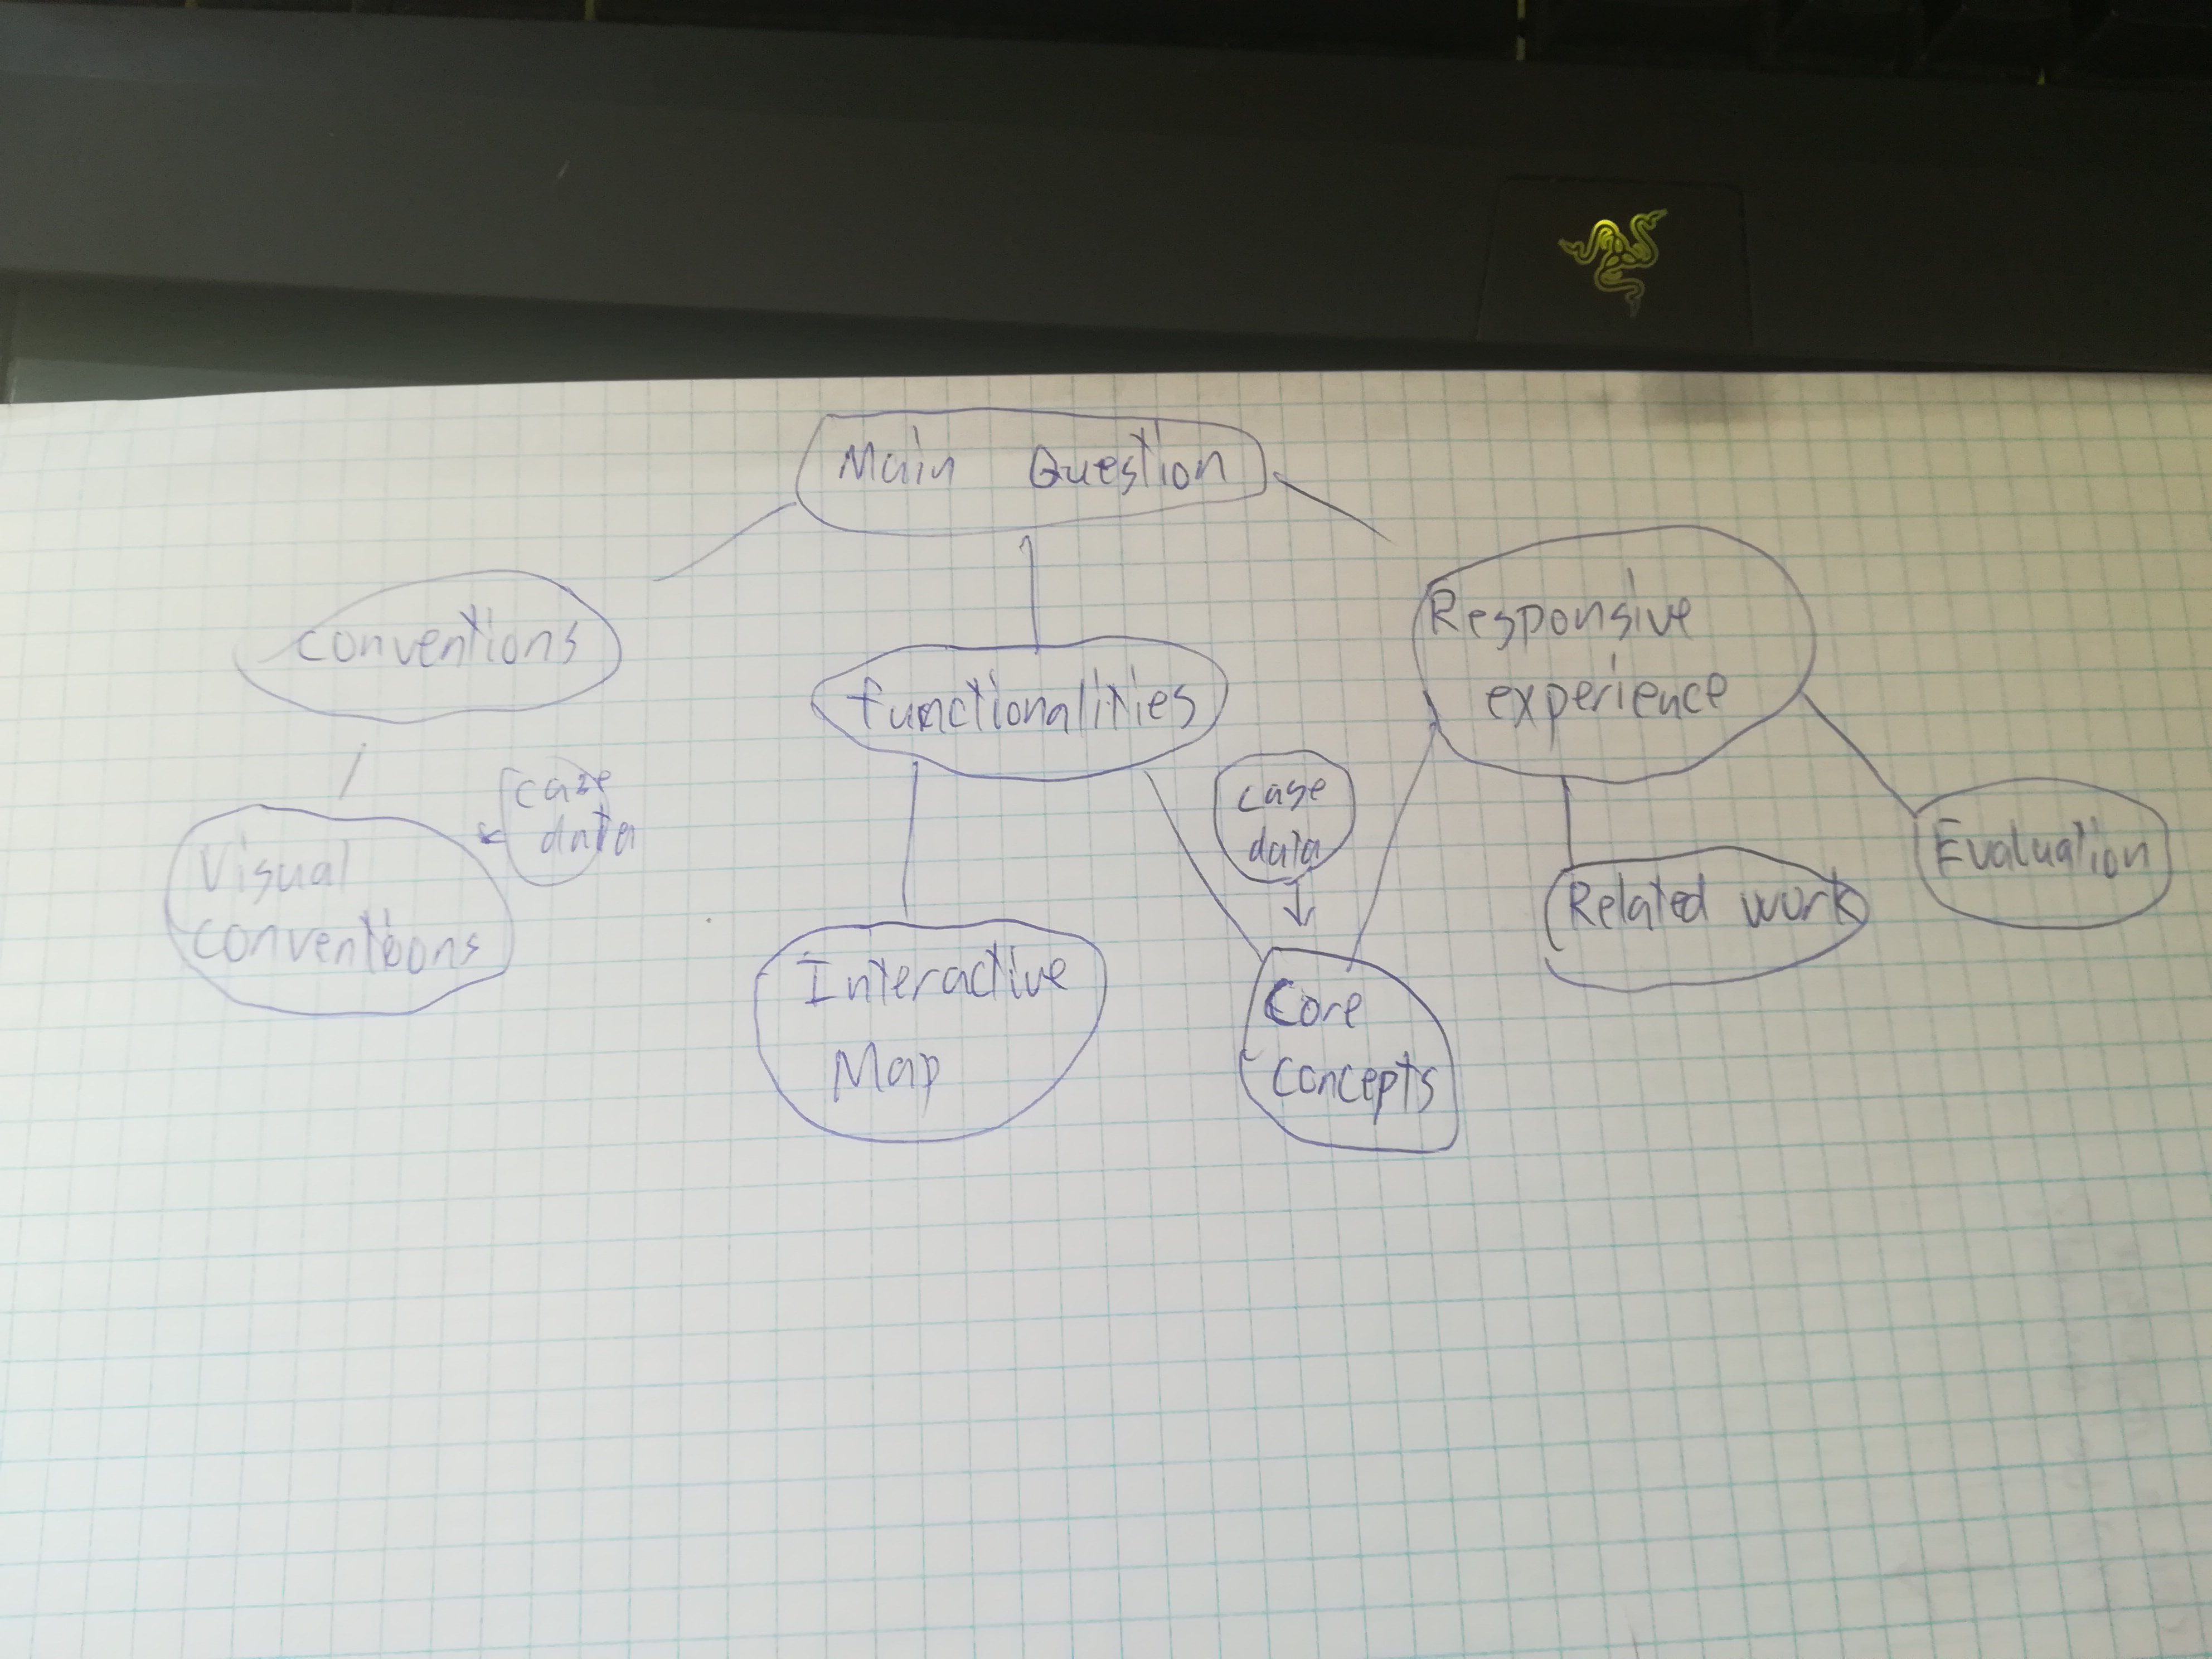
\includegraphics[width=.8\textwidth]{Pictures/Structure}
	\caption{Overview of how the research question gets answered in the first part of the report}
	\label{Structure}
\end{figure}

The rest of the first part is focused on answering the subquestions as illustrated in figure \ref{Structure}. 
The first subquestion is answered through a literature review in chapter x. After the visual conventions have been explained an example of an interactive map gets analysed in chapter x. This is done to understand which functionalities are important for such a map. This is followed by a review of related work in chapter x. Based on the related work and an initial exploration of the data five technical concepts for the tool are created. These are described in chapter x. All of the considerations presented in this part then get collected into the design in chapter x. 

The second part is the development of the tool. In chapter x the building blocks, which the tool is build from, are presented. How these building blocks are put together is then explained in chapter x. Chapter x is an overview of the final product.


The last part starts with an evaluation of the developed tool in chapter x. This is followed by chapter x with a discussion of the tool and how it could be developed further. The last chapter is the conclusion in chapter x 

\fxnote{Update structure and create figure}
